\section{Audio and Heartbeat}
The audio and heartbeat system run concurrently with the rest of the program. On an operating system supporting neither processes nor threads that means using interrupts to stop normal execution and perform tasks on the side.\\
\par
The idea is to configure the hardware to trigger a hardware interrupt at a regular interval. This interrupt is caught by a system called PIC which transforms it into a software interrupt. The software interrupt ID is used as an offset in a vector to look up a function belonging to the engine. At this point, the CPU is stopped (a.k.a: interrupted) from doing whatever it was doing (likely running the 3D renderer), and it started running the interrupt handler which is called an ISR\footnote{Interrupt Service Routine}. We now have two systems running in parallel.

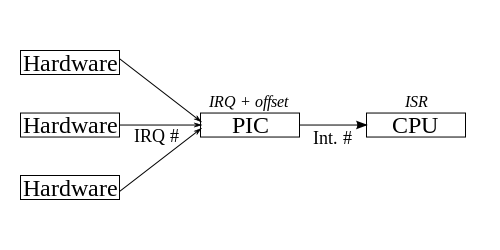
\includegraphics[width=.9\textwidth]{imgs/drawings/irqs/explanation.png}
\par
 Since interrupts keep triggering constantly from various sources, an ISR must make a choice with what should happen if an IRQ is raised while it is still running. There are two ways to go: Decide it needs a "long" time to run and disable other IRQs via the IMR \footnote{Interrupt Mask Register.}. This way to go introduces the problem of discarding important information such as keyboard input or mouse inputs. Or the ISR can decide not to mask other IRQs and do what it is supposed to do as fast as possible, keeping in mind the routine can be stopped (and never resumed).\\
 \par
 Wolfenstein 3D uses the latter approach and keep things in its ISR very small and short. To this effect everything in the audio and heartbeat system is written in assembly and it avoid "heavy" processing.

\subsection{IRQs and ISRs}
The IRQ and ISR system relies on two chips: The Intel 8254 which is a PIT \footnote{Programmable Interval Timers} and the Intel 8259 which is a PIC \footnote{Programmable Interrupt Controller}. The PIT features a crystal oscillating in square waves. On each edges, it decrements its three counters. When a counter hits zero it generate an IRQ. One counter is connected to the buzzer and generate sounds, one counter is connected to the RAM to automatically perform something called "Memory refresh".  The third counters is connected to the PIC. 
\par
\begin{figure}[H]
\centering
 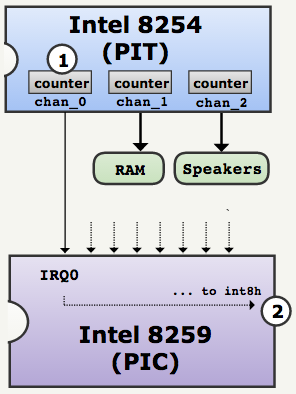
\includegraphics[width=.5\textwidth]{imgs/drawings/heatbeats.pdf}
 \end{figure}
\par

The PIC's hardware IRQ-0 to IRQ-8 are mapped to the Interrupt Vector starting at Offset 8 (resulting in mapping to software interrupts INT08 to INT0F).\\

\par
\begin{figure}[H]
\centering
\begin{tabularx}{\textwidth}{ X X  }
  \toprule
  \textbf{IRQ} & \textbf{Type} \\ \bottomrule
0 & System timer \\
1 & Keyboard controller \\
3 & Serial port COM2 \\ 
4 & Serial port COM1 \\
5 & Line print terminal 2 \\
6 & Floppy controller \\
7 & Line print terminal 1 \\
8 & RTC timer \\
12 & Mouse controller \\
13 & Math co-processor \\
14 & ATA channel 1 \\
15 & ATA channel 2  \\
\bottomrule
\end{tabularx}
\caption{IRQs and routines. Notice \#8 which is associated with the RTC Timer. It usually updates the operating system clock.}
\end{figure}
Using these two chips and placing its own function at Interrupt Vector Table \#8, the engine can stop its runtime at a regular time interval, effectively implementing a subsystem running concurrently with everything else.\\
\par
The engine can decide at what frequency to be interrupted, depending on that type of sound/music it needs to play (digitized sounds are much more taxing than MIDI based sound effects). As a result, three different ISRs can be found at IVT \#8: 
\begin{enumerate}
\item \cw{SDL\_t0ExtremeAsmService} when running at 7000Hz, to play digitized (PCM) sound.
\item \cw{SDL\_t0FastAsmService} when running at 700Hz when playing MIDI music and sound effects.
\item \cw{SDL\_t0SlowAsmService} when running at 140Hz to play sound effects on the beeper via PWM.
\end{enumerate}
\par



\subsection{PIT and PIC}
The PIT chips runs at 1.193182 MHz. That sounds like an odd choice from the hardware designers. The reason of this choice has an uncanny origin. Back in the 1980 when the first IBM PC 5150 was designed, the common oscillator used in television circuitry was running at 14.31818 MHz. Because it was mass produced, it was also very cheap. The decision to use TV oscillator helped to drive the cost of the machine down. Engineers built the PC timer around it, dividing the frequency by 3 for the CPU (that is why the Intel ran at 4.7Mhz), dividing by 4 to 3.57Mhz for the CGA video card. By logically ANDing these signals together a frequency equivalent to the base frequency divided by 12 was created. This frequency is 1.1931816666 MHz. By 1991 the oscillator were much cheaper and could have used any frequency but backward compatibility forbidden it.\\
\par


\subsection{Hearbeats}
Each time the interrupt system triggers, before taking care of the audio requests, it run an other small (yet paramound) system. The sole goal of the heartbeat system is to maintain a 64 bits variable: \cw{TimeCount}.\\
\par
\begin{minipage}{\textwidth}
\lstinputlisting[language=C,morekeywords={longword}]{code/timecount.c}
\end{minipage}
\par
It is updated at a rate of 70 units per seconds (to match VGA update rate of 70Hz). These units are called "ticks". Depending on how fast the audio system runs (from 150Hz to 7000Hz) it adjust how much it should increase \cw{TimeCount}.\\
\par
Every system in the engine uses this variable to pace itself. The renderer will not start rendering a frame until at least one tick has passed. The A.I system express action duration in tick units. The input sampler checks for how long a key was pressed, the list goes on. Everything interacting with humans uses \cw{TimeCount}.\\

\subsection{Audio system}
The audio system is complex because of the fragmentation of the audio devices it can deal with. This was a time before Windows 95 harnessed all audio cards under DirectSound common API. Each development studio had to write their own abstraction layer and id Software was not exception. At high level, the Sound Manager offers a few simple method.\\
\par
\begin{minipage}{\textwidth}
\lstinputlisting[language=C,morekeywords={longword}]{code/sound.h}
\end{minipage}
\par
But under this clean interface lays a maze of functions directly accessing the I/O port of four sound ouputs: Adlib, SoundBlaster, Buzzer and Disney Sound source.




\subsection{Music}
Playing music is not too messy since only PC equipped with a FM synthesizer can play tracks (a.k.a: With an Adlib or a SoundBlaster inside). Because SoundBlaster made its programming interface compatible with Adlib there is only one code path to both cards. There is not a lot of magic here since this part uses a piece of hardware designed and dedicated to this specific task. There are however a few cool tricks.\\
\par
The music system streams data to the sound cards.  Musics in the 90s were not in digitalized format like CD or MP3 nowadays (that would have taken too much storage space and bandwidth). Instead musics are stored as series of notes played on channels together simulating instruments. The format used is close to the notorious MIDI but with a few variation and is called IMF\footnote{Id Music Format}. It is proprietary to id software and designed with OPL2 in mind (the raw format is exactly what is sent to the Adlib/Soundblaster synthesizer with no transformations). IMF has a hardcoded playback rate and music notes are played at 700 Hz.\\
\par
Hardware limitations dictated certain aspects of the design of the musics. The FM synthesizer (OPL2) has 9 channels (a.k.a instruments). Yet the composer, Bobby Prince, was asked to use only channel 1 to 8 for the musics. This little trick allows to multiplex music and sound effects on an AdLib cards since it leave channel 0 available at all time (the SoundBlaster plays sound differently).\\



\subsubsection{Disney Sound sound system: PCM}
The Disney Source has a simple design.After setting the bitrate, its 6 bits DAC will consume PCM bytes from an internal 16 bytes deepFIFO and turn them into sound via its integrated loud speaker.\\ 
\par
Hence every times it awakes, the audio system simply read the parallel port to check if the FIFO has a free spot. It if does it write as many bits as possible until full and returns. When the FIFO gets empty, the Disney Sound source stops making noise.\\
\note{This part should be improved. Read "Disney Sound Source programming manual.""}




\subsubsection{AdLib/Soundblaster music programming}
\par
Programming the OPL2 output is esoteric to say the least. Adlib and Creative did publish SDK but they were very expensive. Documentation was sparse and often cryptic. Today it is almost impossible to find. Luckily only two ports are used, one to select the card register and the other one to read/write data.\\
\par
\begin{minipage}{\textwidth}
\lstinputlisting[language=C,morekeywords={longword}]{code/audio_ports.c}
\end{minipage}
\par
When the AdLib first got released in 1986, developers were instructed to send music  to these ports "as fast as possible". At 4.77Mhz a PC was not able to outpace the Adlib. But as CPU got faster issues started to arise. User manual were amended.\\
\par

\begin{fancyquotes}
After writing to the register port, you must wait twelve cycles before sending the data; after writing the data, eighty-four cycles must elapse before any other sound card operation may be performed\footnote{http://www.oldskool.org/guides/oldonnew/sound}.
 \bigskip \\
 Alternatively you can issue one IN instruction.
 \bigskip \\
 \end{fancyquotes}
\\
\par
Later, reliable specs were published.\\
\par
\begin{fancyquotes}
Wait three point three (3.3) microseconds for the address, and twenty-three (23) microseconds for the data.\\
 \end{fancyquotes}
 
\par





\subsubsection{Adlib sound system}
Adlib only has a FM synthesize and it is used to play sound on its Channel 0. This is done the same way music as previously described so it is not discussed further here.




\subsection{SoundBlaster sound system}
The audio configurations are many. The sound settings screen illustrate well how complicated it is.
\par
\begin{figure}[H]
\centering
 \fullimage{audio/audio_settings.png}
 \end{figure}
\par
Sound effects and Digitized sounds are actually the same thing. Sound effects are stored in three formats. Once for PC Speaker, once for Adlib and once for SoundBlaster/Disney Sound Source. The sounds were stored in the same order and separated by format by Muse. The audio archive is using id software proprietary format, AudioT. The header generated by Muse is self explanatory.\\

\par
\begin{minipage}{\textwidth}
\lstinputlisting[language=C,morekeywords={longword}]{code/muse_header.c}
\end{minipage}
\par
Strangely, only PC speaker and Adlib sounds are stored in the \cw{AUDIO.*} files, the digitized sound are in the\cw{VMSWAP.*} archive. As a result, offset \cw{STARTDIGISOUNDS} is never used.\\
\note{Question for the developers: Why not include the sb sounds in AudioT?} 
\par



\subsubsection{Beeper sound system: PCM}
Digitized sounds were the new rage in the early 90s. They gave SoundBlaster an edge over Adlib which made them the de-facto standard. These sounds are stored in PCM\footnote{Pulse-Code modulation} format where sound is sampled at a certain rate, over channels (left and right) at a certain precision (usually 16 bits values).\\
\par
That encoding it is enough to reconstruct a sound on a loud speaker (as a reference point audio CD uses 44Hz, 16 bits stereo sampling).\\
\par

Wolfenstein 3D sounds are stored in 8 bits precision on a single channel at 7000 Hz.\\



\par
\bu{Stereo system :}\\
\par

On a "high-end" stereo SoundBlaster Pro with left and right channel, the sound is more elaborated: The sound source is rotated with the same formula as the raycaster. Using SOH-CAH-TOA. Intensity is hardcoded 0-15:\\
\par
\begin{figure}[H]
\centering
 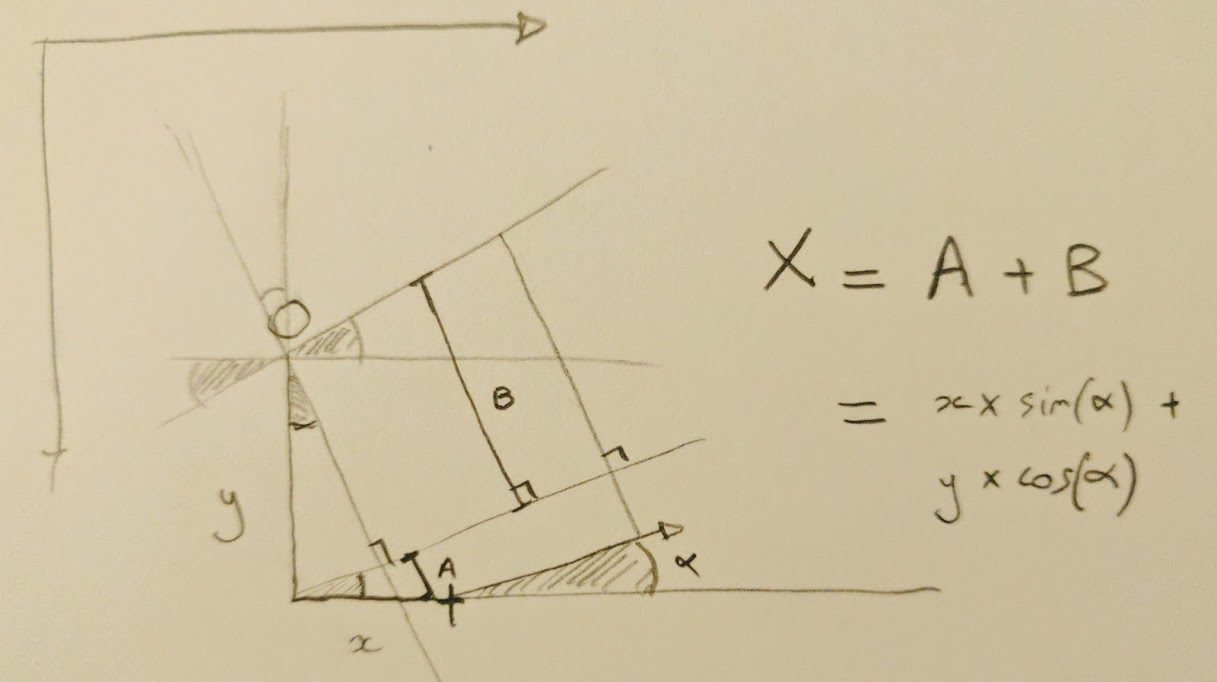
\includegraphics[width=\textwidth]{imgs/drawings/audio_y_rotate.png}
 \end{figure}
 \par
 \begin{figure}[H]
\centering
 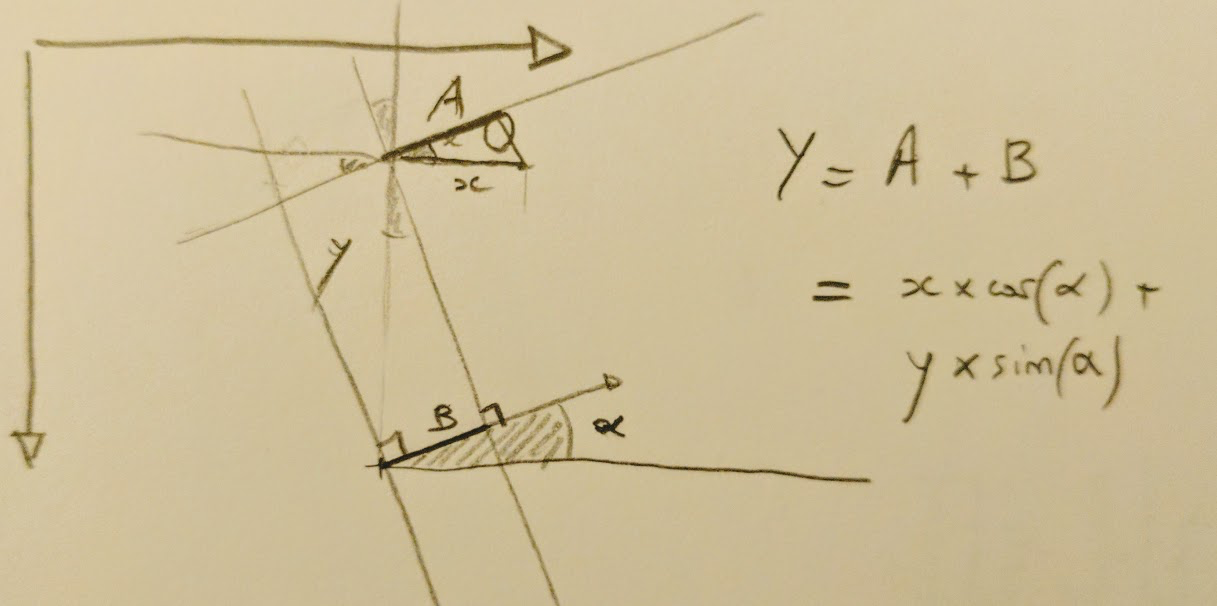
\includegraphics[width=\textwidth]{imgs/drawings/audio_x_rotate.png}
 \end{figure}
\par
In sound part, trivia with a bunch of translations: https://www.gamefaqs.com/pc/564603-wolfenstein-3d/faqs/1824\\
Talk about morse code in episode 3 and 6.\\
\par
\bu{Trivia :} Plugging a sound blaster card was not enough to hear sound. This was before "plug \& play" was introduced by Windows 95. The use had to write a special line in the startup command of the PC (\cw{autoexec.bat}).\\
\par 
\begin{minipage}{\textwidth}
\lstinputlisting[language=C]{code/soundblasterconf.c}
\end{minipage}
\par
This line defines a variable \cw{BLASTER} which the engine retrieve at runtime with \cw{getenv}. \cw{A} tells what port the card is using. \cw{I} gives away the interrupt vector it is associated with. Finally \cw{D} gives the DMA channel to use for data transfer. Of course for all this to work the sound card had to be configured accordingly with jumpers connectors.

 
\subsubsection{Sound on PC Speaker}
The hardware chapter described a problem for sound effects. The default PC speaker can only generate square waves resulting in long beep. But of course hackers found a way to make more than it was meant to.

\par
 \begin{fancyquotes}
  The PC speaker is normally meant to reproduce a square wave via only 2 levels of output (the speaker is driven by only two voltage levels, typically 0 V and 5 V). However, by carefully timing a short pulse (i.e. going from one output level to the other and then back to the first), and by relying on the speaker's physical filtering properties (limited frequency response, self-inductance, etc.), the end result corresponds to intermediate sound levels. This effectively allows the speaker to function as a crude 6 bit DAC,[5] thereby enabling approximate playback of PCM audio. This technique is called pulse-width modulation (PWM).
 \end{fancyquotes}
\par
  It gave surprisingly good results such as in Monkey Island music.\footnote{https://www.youtube.com/watch?v=a324ykKV-7Y}\\
  \par

\begin{verbatim}
"http://www.shikadi.net/moddingwiki/Inverse_Frequency_Sound_format"
\end{verbatim}




  \par
The programming trick is to use another part of the PIT chipset. Counter 0 i used to trigger the audio system. Counter 1 cannot be used (it is used to refresh the RAM periodically). Counter 2 however is directly connected to the PC Speaker. The trick is to set this timer to one-shot mode (Mode 1) and program how long to play a square wave. \\
\par At every input one sound sample value was read, converted to timer control value, programmed to timer (starting the pulse). This trick allowed around 6 bits sample resolution / dynamics (or even slightly more with some tricks). When the sample rate was high enough, you can’t hear the high frequency noise on the signal.\\
TODO: Drawing of PWM
\par
\begin{figure}[H]
\centering
\begin{tabularx}{\textwidth}{ X X  }
  \toprule
  \textbf{Mode} & \textbf{Type} \\ \bottomrule
1 & Hardware Re-triggerable One-shot\\
2 & Rate Generator\\
3 & Square Wave Generator\\
4 & Software Triggered Strobe\\
5 & Hardware Triggered Strobe\\
\bottomrule
\end{tabularx}
\caption{Available mode of a PIT counter.}
\end{figure}
Programming the PIT allow to approximate a sinusoid with square waves.
\par
\begin{figure}[H]
\centering
 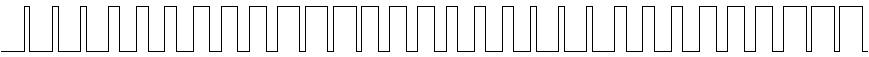
\includegraphics[width=\textwidth]{imgs/drawings/pwm/sinuois.png}
 \caption{The original sound.}
 \end{figure}
\par

\par
\begin{figure}[H]
\centering
 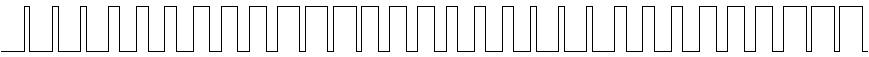
\includegraphics[width=\textwidth]{imgs/drawings/pwm/pwm_approximation.png}
 \caption{The same sound approximated with PWM.}
 \end{figure}
\par


\bu{Hidden feature :} The source code features an audio code path that was never allowed to ship. It can play digitized sound via the PC Speaker.\\

\par 
\begin{minipage}{\textwidth}
\lstinputlisting[language=C]{code/sound_fork.c}
\end{minipage}
\par
Notice the \cw{SDL\_PCPlaySample} path allowing PCM to be played on the buzzer. This codepath was never enabled in shipping product.\\
\par
\footnote{You can hear the difference on youtube: "Wolfenstein 3D Hack - Digitized PC Speaker Sound Effects" at https://www.youtube.com/watch?v=1BtlsjJRnFU}.\\
\par
\note{Why was this never shipped?}







\section{User inputs}
In an era before Microsoft harnessed all input under DirectInput API with Windows 95, all inputs had to be gathered manually. It involves talking directly to the hardware, in the vendor's protocol on a physical port. The keyboard is plugged on physical port PS/2, the mouse uses physical Serial Port and the joystick is plugged on a game port on the SoundBlater (this was almost the only way to get a Joystick port).





\subsection{Keyboard}









\subsection{Mouse}
A driver has to be lowed at startup for the mouse to operate. DOS has a default one.\\
\par 
\begin{minipage}{\textwidth}
\lstinputlisting[language=C]{code/mouse.sys.c}
\end{minipage}
The driver takes almost 5KB of RAM. With the driver loaded all interactions happen with software interrupt 0x33. The interface works with request issued in register AX and response issued in registers CX, BX and DX. With Borland compiler syntactic sugar it is easy to write with almost no boilerplate (notice direct access to registers thanks to \_AX and co special keywords.\\
\par
\begin{minipage}{\textwidth}
\lstinputlisting[language=C]{code/mouse_request.c}
\end{minipage}
\par
\begin{figure}[H]
\centering
\begin{tabularx}{\textwidth}{ >{\hsize=.5\hsize}X  >{\hsize=.5\hsize}X  X }
  \toprule
  \textbf{Request} & \textbf{Type} & \textbf{Response} \\ \bottomrule
AX=0 & Get Status & AX = FFFFh : available. AX Value = 0 : not available\\
AX=1 & Show Pointer & \\
AX=2 & Hide Pointer & \\
AX=3 & Mouse Position & CX = X Coordinate, DX = Y Coordinate\\
AX=3 & Mouse Buttons & BX = 1 Left Pressed, BX = 2 Right Pressed, BX = 3 Centre Button Pressed\\
AX=7 & Set Horizontal Limit & CX=MaxX1 DX=MaxX2\\
AX=8 & Set Vertical Limit & CX=MaxY1 DX=MaxY2\\
\bottomrule
\end{tabularx}
\caption{Mouse request/response.}
\end{figure}
\par









\subsection{Joystick}
\par
\begin{minipage}{\textwidth}
\lstinputlisting[language=C]{code/joystick.c}
\end{minipage}
\par



\begin{figure}[H]
\centering
\begin{tabularx}{\textwidth}{ >{\hsize=.5\hsize}X X  }
  \toprule
  \textbf{Bit Number} & \textbf{Meaning} \\ \bottomrule
0 & Joystick A, X Axis \\
1 & Joystick A, Y Axis \\
2 & Joystick B, X Axis \\ 
3 & Joystick A, Y Axis \\
4 & Joystick A, Button 1 \\
5 & Joystick A, Button 2 \\
6 & Joystick A, Button 1 \\
7 & Joystick B, Button 2 \\
\bottomrule
\end{tabularx}
\caption{Joystick sampling bit meaning.}
\end{figure}
\par







